\xchapter{Avaliação da disponibilidade dos softwares científicos de análise estática}
{Este capítulo apresenta a avaliação e caracterização dos softwares científicos
de análise estática de código fonte quanto à sua disponibilidade ou
sustentabilidade técnica, ou seja, a capacidade de perdurar, de continuar
disponível no futuro.}
\label{caracterizacao-ferramentas}

% Introduction
% Background
% Experimental Setup (hipoteses / design)
% Results (data analysis)
% Discussion
% Threats to validity
% Conclusions

Muitos estudos em engenharia de software sofrem de dificuldades de repetição
\cite{Tang2016}, uma prática importante para aumentar a validade científica dos
estudos e seus resultados. {\it Repetição} é a atividade de refazer exatamente
o que outra pessoa fez usando os artefatos originais, a disponibilidade de
código fonte é o requisito mínimo para possibilitar tal prática.

Avaliar e caracterizar a disponibilidade dos {\it softwares cientificos}
publicados em conferências de engenharia de software, com especial atenção à
disponibilidade do seu código fonte, é útil para evidenciar o quão possível é
repetir tais estudos e assim aumentar a validade em seus resultados.

Sabe-se que artigos que citam o desenvolvimento de scripts ou protótipos
apresentam chance próximo a nulo de ter estes artefatos disponíveis
publicamente e terem seu código fonte acessível. A replicabilidade tende a cair
com a idade do paper, uma das razões é que as páginas web onde os softwares e
possivelmente dados são publicados tem uma grande chance de se tornarem
indisponíveis ao passar do tempo \cite{robles2010replicating}.

O recente Dagstuhl Manifesto \cite{allen2017engineering} indica como futura
direção de pesquisa quantificar a disponibilidade de softwares científicos, e
sugere a seguinte questão de pesquisa: Na literatura científica publicada, como
as taxas de softwares disponíveis, executáveis, e escondidos ({\it hidden
software}) mudam ao longo do tempo?

Alinhado à esta sugestão de investigação, o atual trabalho define como objetivo
geral avaliar a disponibilidade dos softwares científicos publicados em
conferências de engenharia de software e assim evidenciar o quanto tais estudos
sofrem com dificuldades de repetição.

Esta avaliação e caracterização será focada em publicações da área de análise
estática de código fonte visto que seria inviável no escopo deste trabalho
englobar todas as áreas de pesquisa da engenharia de software.

A área de análise estática de código fonte possui carência de estudos avaliando
suas ferramentas, desta forma conseguiremos contribuir com esta área ao mesmo
tempo que exploramos o quanto os pesquisadores publicando softwares nesta área
publicam e disponibilizam seus softwares contribuindo para a divulgação dos
resultados e proporcionam repetição dos seus estudos.

\section{Planejamento do estudo}

\subsection{Seleção de softwares científicos}

Selecionamos softwares via {\it revisão estruturada}, um processo disciplinado
para busca e seleção de softwares de um domínio específico publicados em
artigos acadêmicos a partir de critérios bem definidos, de forma que seja
possível a reprodução do estudo por parte de pesquisadores interessados.

A revisão estruturada difere da revisão e do mapeamento sistemático
\cite{Kitchenham2007} por ser um processo mais simples e menos rígido, onde o
resultado final é um conjunto de softwares, enquanto no mapeamento ou na
revisão sistemática há um esforço em caracterizar os artigos analisados o mesmo
não ocorre na revisão estruturada, onde o esforço está em caracterizar os
softwares científicos.

A revisão estruturada é organizada em três atividades de (1) busca de artigos
(definição das fontes, obtenção dos artigos nas fontes), (2) filtro (definição
de critérios de busca, definição de script de busca) e (3) seleção de artigos
com publicação de softwares. Estas atividades estão representadas na Figura
\ref{figura-revisao-estruturada}.

\begin{figure}[h]
  \center
  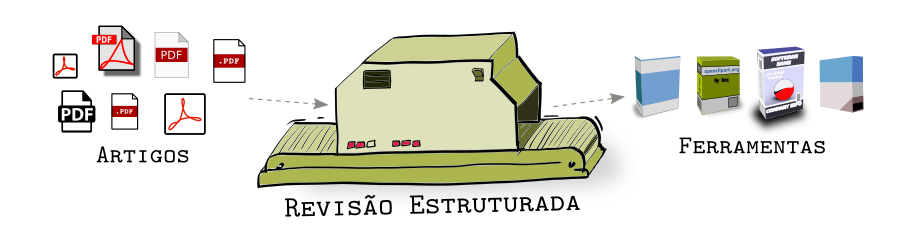
\includegraphics[scale=0.21]{imagens/revisao-estruturada.png}
  \caption{Atividades da revisão estruturada}
  \label{figura-revisao-estruturada}
\end{figure}

O resultado final da revisão estrutuda é um conjunto de softwares científicos e
informações sobre em qual artigo foi publicado, qual conferência e ano o artigo
foi publicado e em quais fontes o software pode ser obtido, geralmente páginas
web, repositórios de código fonte ou outros endereços na internet. Cada
atividade da revisão estruturada é detalhada à seguir:

\begin{description}

  \item[(1) Busca]
    Na primeira atividade da revisão estruturada são definidas as fontes de
    entrada, estas fontes são conferências que abordam o tema de interesse do
    estudo, e que apresentam um grande potencial de encontrar softwares do
    domínio de aplicação desejado, neste estudo o interesse está em softwares
    de análise estática de código fonte, portanto as conferências selecionadas
    serão aquelas com potencial de se encontrar softwares deste domínio de
    aplicação. Esta primeira atividade deve incluir o maior número possível de
    ediçoes possível de cada conferência selecionada, para cada edição são
    copiados localmente todos os artigos em formato PDF para posterior filtro
    na atividade 2.

  \item[(2) Filtro]
    A segunda atividade da revisão estruturada realizada em cima de todo o
    conjunto de artigos selecionados na etapa anterior é um filtro automático
    que busca em todo o conteúdo dos artigos os termos de interesse, estes
    termos devem ser pensados em relaçao ao domínio de aplicação desejado,
    devem ser abrangentes a fim de evitar falsos negativos, ou seja, deixar de
    fora qualquer artigo que tenha o mínimo de indício sobre publicação de
    software de análise estática, mesmo que não publiquem, a atividade seguinte
    irá identificar esses falsos negativos deixando-os de fora do resultado
    final da revisão. Os seguintes termos serão utilizados neste filtro:

    \begin{verbatim}
      "tool" OU "framework"; E
      "download" OU "available"; E
      "http" OU "ftp"; E
      "static analysis" OU "parser".
    \end{verbatim}

    Esses termos devem encontrar artigos com publicação de softwares
    científicos do domínio de análise estática de código fonte com
    disponibilidade para {\it download}, seja binário ou código fonte,
    a serão aplicados automaticamente com auxílio de um script desenvlvido
    durante este trabalho de pesquisa, detalhes deste script, outros artefatos,
    e onde obtê-los pode ser encontrado no Apêndice
    \ref{reproducibilidade-do-estudo}.

  \item[(3) Seleção]
    A terceira e última atividade da revisão estruturada identifica se cada
    artigo resulta, de fato, em publicação de software científico do domínio de
    aplicação desejado. Esta seleção é feita a partir de uma leitura
    superficial do artigo em busca de indícios de que o artigo publica de fato
    algum software.

    Nesta etapa cada artigo é lido, inicialmente apenas introdução, resultados
    e conclusão com o objetivo de identificar se o artigo publica software
    científico e indica onde obter uma cópia do software. Quando esta leitura inicial
    não é suficiente para identificar se há publicação de software, outras seções são
    lidas, alguns artigos descrevem a implementação do software em seções específicas,
    outros indicam detalhes do software ao longo de todo o texto. Softwares científicos
    que sejam mais abrangentes do que apenas análise estática de código fonte
    mas que contenham esta função em seu conjunto também são selecionados.

\end{description}

Ao final das 3 atividades da revisão é gerado como saída um conjunto de
softwares científicos de análise estática de código fonte, para cada software
teremos o nome, uma breve descrição e em qual artigo o software foi publicado.

\subsection{Quantificação da disponibilidade dos softwares científicos}

Avaliamos os softwares científicos de análise estática de código fonte
selecionados na revisão estruturada em relação à sua disponibilidade, dois
aspectos foram levados em conta nesta avaliação, um relacionado à como o artigo
apresenta e disponibiliza o software científico e o outro relacionado a como o
software está de fato disponível, ou seja, se a fonte informada para obtenção
está funcional ou não.

O primeiro aspecto relacionado à como o artigo disponibiliza o software
científico será caracterizado entre uma das seguintes opções:

\begin{itemize}
  \item Artigo não indica onde obter o software:\\
    {\it O artigo não indica fonte para obtenção do software}
  \item Fonte para obtenção do software indisponível:\\
    {\it O artigo indica fonte mas encontra-se inacessível, fora do ar ou com erros}
  \item Software disponivel, binários ou código fonte\\
    {\it A fonte indicada está disponível e acessível publicamente}
\end{itemize}

Este primeiro aspecto tem a importância de mostrar quantos artigos falham em
não informar ao leitor qual ou quais são as fontes para obtenção dos artefatos
de software produzidos no estudo. A fonte indicada será acessada a fim de
identificar se está funcional e se é possível obter uma cópia do software.
Este é um requisito fundamental para conseguir responder positivamente às
questões apresentadas no manifesto Dagstuhl \cite{allen2017engineering}:

\begin{quote}
  O software que nós usamos e produzimos no contexto acadêmico é sustentável?
  Temos certeza de que podemos reproduzir métodos de pesquisas anteriores no
  futuro, tendo em vistas mudanças arbitrárias no contexto tecnológico?
  Podemos adaptar de forma incremental o software acadêmico para aproveitar
  oportunidades emergentes, sem perda de reprodutibilidade e sem custos
  proibitivos?
\end{quote}

%Mesmo que o autor tenha disponibilizado fontes para obtenção dos artefatos produzidos,
%o fato de não informarem a fonte inviabiliza, ou ao menos dificulta, bastante
%pesquisadores interessados em repetir ou reproduzir os resultados de tais estudos.

É claro que não podemos responder à todas estas questões com a caracterização deste
primeiro aspecto em relação à disponibilidade dos softwares, ou, sua sustentabilidade
técnica, a capacidade de perdurar e continuar disponível no futuro. Mas este é o requisito
mínimo necessário para conseguir responder tais questões, sem ele é extremamente difícil
conseguir resposta para tal.

O segundo aspecto diz respeito à como o software está disponível, é um nível de
detalhe sobre o primeiro aspecto, os softwares caracterizados como disponíveis
no primeiro aspecto serão detalhados aqui, informando de que forma estão
disponíveis, se código fonte, binários de forma gratuita, ou disponíveis apenas
comercialmente.

\begin{itemize}
  \item Código Aberto ({\it Open Source}):\\
    {\it A ferramenta é livre e o código fonte está disponível}
  \item Grátis ({\it Free}):\\
    {\it A ferramenta é grátis mas o código fonte não está disponível}
  \item Comercial:\\
    {\it A ferramenta está disponível mediante pagamento}
\end{itemize}

Lembrando, apenas os softwares caracterizados no primeiro aspecto como
{\it``Software disponivel, binários ou código fonte''} serão detalhados aqui.
Esse segundo aspecto toma como base o trabalho de \citeonline{Novak2010} em que
propõe uma taxonomia e um conjunto de dimensões para caracterização de
ferramentas de análise estática, uma das dimensões para caracterização
é esta relacionado à como o software é disponibilizado.

Os softwares caracterizados como {\it ``Código Aberto (Open Source)''}
incluirão qualquer software com código fonte disponível, mesmo sem licença
definida, sabemos que isto contraria as definições de software {\it livre} e
{\it open} da Free Software
Foundation\footnote{\url{https://www.gnu.org/philosophy/free-sw.html}} e Open
Source Initiative\footnote{\url{https://opensource.org/osd}}, respectivamente,
mas será feito assim pois o acesso ao código fonte é a característica de
interesse neste estudo, com ele é possível estudar o conhecimento empregado nos
softwares, bem como repetir o estudo original utilizando ou executando tal
código quando necessário.

A fonte de informação para a caracterização desses dois aspectos serão os
artigos relacionados aos softwares, código fonte, documentos e site do projeto,
quando disponíveis.

\section{Resultados}

Na {\it revisão estruturada} selecionamos a conferência SCAM - {\it
Source Code Analysis and Manipulation Working
Conference}\footnote{\url{http://www.ieee-scam.org}} e a conferência ASE - {\it
Automated Software Engineering}\footnote{\url{http://ase-conferences.org}},
ambas conferências com largo histórico de publicação sobre análise de
programas e apresentam um alto potencial de encontrar softwares do domínio de
análise estática de código fonte.

A primeira atividade da revisão estruturada -- {\it (1) Busca} -- passa por
todas as ediçoes das duas conferências até o ano de 2015. Todas as trilhas de
ambas as conferências foram incluídas, econtramos nesta atividade 1873 artigos
no total, 346 artigos do SCAM e 1530 artigos do ASE, uma média de 75 artigos
publicados por ano.

\begin{figure}[h]
  \center
  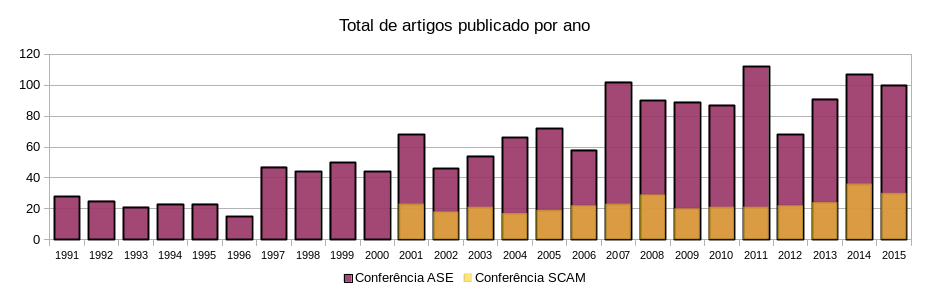
\includegraphics[scale=0.65]{imagens/grafico-artigos-por-ano.png}
  \caption{Gráfico em barras com o total de artigos publicado por ano}
  \label{grafico-artigos-por-ano}
\end{figure}

Até o ano de 1996 a conferencia ASE chamava-se KBSE - {\it Knowledge-Based
Software Engineering Conference} e só a partir de 1997 passou a chamar-se ASE -
{\it Automated Software Conference}. O ano com o maior número de publicações
foi 2011 com um total de 112 artigos, seguido de 2014 com 104, e 2007 com 102,
o ano com o menor número foi 1996 com apenas 15 artigos publicados.

Se compararmos os mesmos períodos de ambas as conferências, entre 2001 e 2015,
é fácil perceber que a conferência ASE publica, no mínimo, 3 vezes mais em
números do que a conferência SCAM, com uma média de 80 e 23 respectivamente.

A segunda atividade da revisão estruturada -- {\it (2) Filtro} -- realizada
neste conjunto total de 1873 artigos resultou em 441, 155 artigos da
conferência SCAM e 286 da conferência ASE.

%44\% do total de artigos da conferência SCAM e 10\% dos artigos do ASE possuem
%os termos indicanos no filtro para uma busca abrangente de publicação de
%ferramentas.

Alguns artigos foram analisados manualmente pois o conteúdo era formado por
imagens de forma que o script de filtro não é possível de processar textos
contidos em imagens, foram artigos do ASE 2004: {\it Adaptable concern-based
framework specialization in UML} e {\it Property-oriented test generation from
UML Statecharts}. Nenhum continha os termos pesquisados.

A terceira e última atividade da revisão estruturada -- {\it (3) Seleção} --
realizada em cima dos 441 artigos selecionou 107 artigos com publicação de
software científico do domínio de aplicação de análise estática de código
fonte, 41 da conferência SCAM e 66 da conferência ASE, os Apêndices
\ref{artigos-do-scam} e \ref{artigos-do-ase} detalham o total de cada
conferência.

Assim, ao final da revisão estruturada encontramos um total de 107 artigos com
publicação de software de análise estática de código fonte, alguns artigos
fazem referência ao mesmo software, estes 107 artigos fazem referência à 105
softwares diferentes, uma lista com todos os softwares e uma breve descrição de
cada um é apresentado no Apêndice \ref{resumo-softwares}.

Todos os artigos indicam o nome do software e apresentam algum nível de detalhe
sobre eles, apesar da busca na atividade -- (2) Filtro -- utilizar termos com o
objetivo de encontrar apenas softwares disponíveis 45 artigos encontrados não
indicam onde encontrar e obter o software.

\begin{table}[H]
\centering
\begin{tabular}{| l | l |}
  \hline
  {\bf Característica}                          & {\bf Número de artigos} \\
  \hline
  Artigo não indica onde obter o software       & 45 \\
  \hline
  Artigo indica fonte para obtenção do software & 59 \\
  \hline
\end{tabular}
\end{table}

Dentre os 1873 artigos, 107 referenciam 105 softwares de análise estática, e
apenas 59 destes indicam uma fonte onde o software pode ser encontrado, 24
destes artigos indicam fontes indisponíveis, todos indicam algum endereço web e
alguns deram endereço não encontrado e outros endereços caem em sites não
relacionados ao software. Outros 35 artigos indicam fonte disponível para
obtenção, todos indicam endereço de um site ou repositório e estão disponíveis,
seja em formato binário apenas ou em código fonte.

\begin{table}[H]
\centering
\begin{tabular}{| l | l |}
  \hline
  {\bf Característica}                          & {\bf Número de artigos} \\
  \hline
  Fonte para obtenção do software indisponível  & 24 \\
  \hline
  Fonte para obtenção do software disponivel    & 35 \\
  \hline
\end{tabular}
\end{table}

Uma avaliação sobre estes 59 softwares que tem sua fonte indicada no artigo
feita para identificar que confirmamos neste contexto se com a idade do paper
as páginas web onde os softwares são publicados tem uma grande chance de se
tornarem indisponíveis ao passar do tempo, a Figura
\ref{softwares-disponivel-por-ano} mostra quantos porcentos do total de
softwares com indicação de fonte estão ainda disponíveis hoje.

\begin{figure}[h]
  \center
  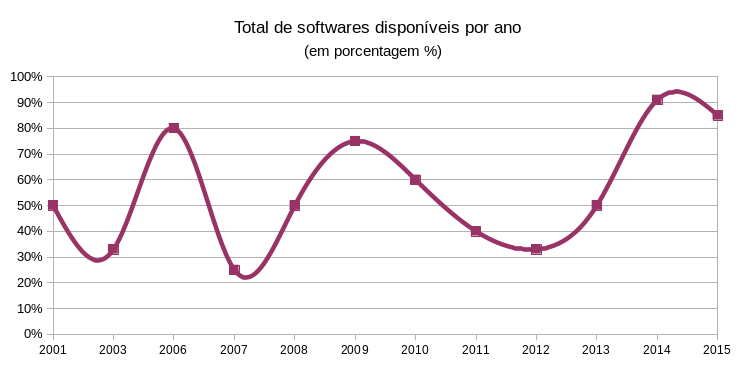
\includegraphics[scale=0.65]{imagens/softwares-disponivel-por-ano.png}
  \caption{Gráfico em linha com o total de softwares disponíveis por ano}
  \label{softwares-disponivel-por-ano}
\end{figure}

Não é possível identificar se há um padrão de crescimento ao longo do tempo com
as amostras analisadas, em 2006 80\% de todos os softwares de análise estática
publicados nas conferências SCAM e ASE estão ainda disponíveis e é possível
obter uma cópia dos softwares livrevemente. Este número cresce em 2014 chegando
a 90\%, e no ano seguinte 2015 começa a cair 85\%. Lembrando que são softwares
publicados em artigos indicando a fonte para obtenção.

Os anos de 2005, 2004, 2002 e anteriores ao ano 2001 não possuem softwares
publicados com fonte indicada no artigo ainda disponível.

Esses 35 softwares com fonte disponível foram avaliados em relação ao segundo
aspecto em respeito à de que forma estão disponíveis.

\begin{table}[H]
\centering
\begin{tabular}{| l | l |}
  \hline
  {\bf Característica}                          & {\bf Número de artigos} \\
  \hline
  ``Código Aberto ({\it Open Source})''         & 32 \\
  \hline
  ``Grátis ({\it Free})''                       & 3  \\
  \hline
  ``Comercial''                                 & 0  \\
  \hline
\end{tabular}
\end{table}

Em outras palavras, de um total de 103 artigos publicando softwares de análise estática de
código fonte, apenas 32 artigos (31\%) estão disponíveis para download com
código fonte, o que nos leva a conclusão que os 71 artigos (69\%) restantes não
podem ser repetidos considerando que disponibilizar o código fonte dos
artefatos de software é o mínimo requisito para possibilitar tal prática.

\section{Ameaças à validade}

Estamos considerando que o código fonte é necessário para repetir um dado
estudo mas pode ser que em alguns casos o estudo possa ser repetido mesmo sem a
disponibilidade do mesmo, isto poderia ser resolvido realizando a repetição
de cada estudo na prática e a partir daí identificar se o código fonte dos
softwares desenvolvidos são requeridos.

A escolha de um domínio de aplicação específico para seleção dos softwares
pode ser um fator de influencia nos resultados obtidos, sendo possível que
o número de artigos com publicação de softwares com código fonte disponível
encontrado não reflita nos outros domínios, os problemas diagnosticados
neste domínio pode não ser verdade em outros domínios, sendo necessário
realizar o mesmo estudo em outros domínios.

A leitura dos artigos na revisão estruturada para identificar se publicam
softwares de análise estática de código fonte, se disponibilizam fonte para
obtenção de tais softwares, e se os softwares são mesmo do domínio de aplicação
de análise estática de código fonte podem ter maior validade se feitos em
par e revisados por outros pesquisadores, neste estudo tudo foi feito pelo
autor deste estudo e não houve revisão por pesquisadores independentes.

\section{Conclusões}

Dos 346 artigos do SCAM e 1533 artigos do ASE analisados na revisão estruturada
apenas 44\% (155 artigos) e 18\% (281 artigos) continham os termos pesquisados
no filtro automático da segunda atividade da revisão, respectivamente.

Deste total apenas 11\% (41 artigos) e 4\% (62 artigos) foram selecionados na
terceira e última atividade da revisão contendo publicação de ferramenta de
análise estática.

Resultando em 103 artigos com publicação de {\it software científico} de
análise estática de código fonte, apenas 35 possuem fonte para obtenção do
software, sendo 32 de código aberto, ou seja, com disponibilidade de
código fonte, e 3 grátis, apenas binários disponível. Ou seja, apenas 31\% dos
artigos com publicação de software disponibilizam o código fonte das mesmas.
Isto significa que 69\% dos artigos com publicação de software de análise
estática de código fonte são potencialmente impossíveis de serem repetidos, já
que os artefatos originais são necessários para tal atividade e o artigo não
disponibiliza o código fonte dos mesmos.

% o artigo com resumo do RESER 2011 diz \cite{knutson2010report}:
% 4) Re-
% search tools are either not available or not usable, so precise
% replication is impractical [1, 2, 8, 18, 19].

Muitos outros aspectos podem ser levados em consideração quando se está
avaliando a capacidade de repetir ou replicar um estudo, aqui avaliamos apenas
a disponibilidade de código fonte dos softwares científicos, mas inúmeros detalhes
pormenores são necessários, tais como: indicar qual versão do software foi
utilizado no estudo, 

No entando, consideramos que nem todos os scripts e código fonte pode
valer o custo de dua publicação, sabe-se que umas das barreiras para publicação
de muitos destes artefatos são as dificldades em tal atividade,
e as objeções a tal prática de ter RR reques um esforço adicional \cite{madeyski2017would},
em muitos
estudos o simples fato de não possuir código disponível pode não levar
a problemas para alcançar a meta final que é aumento da validade do estudo,


Todas as atividades e artefatos produzidos neste estudo estão documentados em
repositório público no
Github\footnote{\url{http://github.com/joenio/dissertacao-ufba-2016}}, o
Apêndice \ref{apendice-revisao-estruturada} traz mais informações.

%, uma lista completa e
%o endereço de cada edição onde os artigos foram obtidos está documentado no
%Apêndice \ref{edicoes-conferencias}

% IDEIA!
% levantar ano de publicação do artigo para cada software e
% calcular por quanto tempo cada software está disponível,
% com isso verificar se há um padrão, ou seja, se publicações
% mais antigas possuem softwares não-disponíveis, obsoletos,
% etc...
